%!TEX root=main.tex
\vspace{-5pt}
\section{Introduction\label{sec:intro}}
% one for each key finding: a) many features deemed to be of importance to VQSs by domain experts, not all supported by present-day VQSs b) sketch is inefficient, perhaps explaining why present-day VQSs are not popular c) identify 3 typical workflows involving various sensemaking modalities in different proportions, depending on the application
Line charts are commonly employed during data exploration---the 
intuitive connected patterns 
often illustrate complex underlying processes
and yield interpretable and visually compelling data-driven
narratives. 
To discover patterns in line charts,
analysts construct them
using toolkits like \texttt{ggplot} or \texttt{matplotlib},
or visualization construction interfaces
like Excel or Tableau, specifying 
{\em exactly} what they want to visualize.
For example, when trying to find celestial objects 
corresponding to supernovae, which have a specific pattern
of brightness over time, astronomers 
individually inspect the corresponding line chart 
for each object (often numbering in the hundreds) 
until they find ones that match the pattern. \ccut{Similarly, when trying to infer relationships between two physical properties for different subsets of battery electrolytes, scientists need to individually visualize these properties
for each subset (out of an unbounded number of such subsets)
until they identify relationships that make sense to them.} 
This process of manual exploration of
large numbers of line charts 
is not only error-prone, but also overwhelming for 
analysts.
%, not only for time series but also for understanding the relationships between multiple measures variables.

% From high-throughput genome sequencing,
% to multi-resolution astronomical imaging telescopes,
% to at-scale physical testing of battery candidates,
% many fields of science and engineering
% are facing an increasing availability of
% large volumes of complex data~\cite{AustinNothaft2015,Demchenko2013},
% holding the key to some of the most pressing
% unanswered scientific questions of our time,
% such as: How does a treatment affect the
% expression of a gene in a breast cancer cell-line?
% Which battery components have sustainable levels
% of energy-efficiency and are safe and cheap to
% manufacture in production?
% While data analysis is central to a scientist's
% knowledge discovery process, scientists
% often lack the extensive experience to deal
% with data of this scale and complexity
% in a way that can facilitate rapid insight discovery~\cite{Kersten2011}.with the system automatically traversing all potential visualization candidates to find those that match the specification
\par To address this challenge, 
there has been a large number of papers 
dedicated to building {\em Visual Query Systems} (VQSs), 
that allow users to specify 
desired visual patterns 
via an interactive interface~\cite{mohebbi2011google,Hochheiser2004,wattenberg2001sketching,Siddiqui2017VLDB,ryall2005querylines,correll2016semantics,Mannino2018,Eichmann2015,Holz2009}. 
This interactive interface is one with 
a sketching canvas
where users can draw a pattern of interest,
with the system automatically traversing 
all potential visualization candidates 
to find those that match the specification. 
Since the intent of a sketch can be ambiguous, 
some work has developed mechanisms to
enable users to clarify 
how a sketch should be interpreted~\cite{ryall2005querylines,correll2016semantics,Mannino2018,Eichmann2015,Holz2009}. 

\par 
While this intuitive 
specification interface 
seems to be a promising solution 
to the problem of painful manual exploration of visualizations, 
to the best of our knowledge, VQSs are not very commonly used in practice. 
{\em Our paper seeks to bridge this gap 
to understand how VQSs can actually be used in practice, 
as a first step towards the broad adoption of VQSs in data analysis}.
Unlike prior work on VQSs,
we set out to not only evaluate VQSs in-situ on
real problem domains, but also involve participants
from these domains in the VQS design. 
We present findings from a series of interviews, 
cognitive walkthroughs, participatory design, 
and user studies with scientists from three different domains---{\em astronomy, genetics,} and {\em material science}---over the course of 
a year-long collaboration. 
These domains were selected to capture 
a diverse set of goals 
and datasets wherein VQSs can help address 
important scientific questions, such as: 
How does a treatment affect the expression 
of a gene in a breast cancer cell-line? 
Which battery components have sustainable 
levels of energy-efficiency and are safe and 
cheap to manufacture in production?

\par Via cognitive walkthroughs and interviews, we first identified challenges in existing data analysis workflows in these domains
that could be potentially addressed by a VQS. Building on top of an existing, open-source VQS, \zv~\cite{Siddiqui2017,Siddiqui2017VLDB}, we collaborated closely with our participants to gather feedback and iterate on VQS feature designs,
over the course of a year, culminating in a new enhanced VQS, \zvpp. We organized these features into a taxonomy of VQS functionalities, \change{involving three sensemaking processes inspired by Pirolli and Card's notional model of analyst sensemaking~\cite{Pirolli}. The sensemaking processes include top-down pattern specification (translating a pattern ``in-the-head'' into the form of a visual query), bottom-up data-driven inquiries (querying or recommending based on data), and context-creation (navigating across different collections of visualizations).} We find that prior VQSs have focused largely on top-down processes, while largely ignoring the other two processes that are crucial for the needs \change{in} all three domains.

\par 
To study how various VQS features 
are used in practice, 
we conducted a final evaluation study with nine participants 
using our final VQS prototype, \zvpp, 
to address their research questions 
on their own datasets. 
In a 1.5-hour user study, participants were able to 
gain novel scientific insights, 
such as identifying a star with a transient pattern 
that was known to harbor a Jupiter-sized planet 
and finding characteristic gene expression profiles confirming the results of a related publication.\techreport{, and discovering that the dip in an astronomical light curve is caused by saturated imaging equipment overlooked by the existing error-detection pipeline.} \techreport{Participants also gain additional insights about their datasets, including debugging mislabeled features and uncovering erroneous data preprocessing procedure applied to a collaborator's dataset.} 
%that goes from a pattern in-the-head to a desired visualization 

\par By analyzing the evaluation study results, we discovered that sketching a pattern \change{for querying} is often ineffective. This is due to the fact that sketching makes the problematic assumptions that users know the pattern that they want to sketch and are able to sketch it precisely. Instead, participants typically opted for other means of pattern specification---one common mechanism was to drag-and-drop a \change{recommended} pattern onto the canvas, and then modify it (e.g., by smoothing it out). However, most VQSs do not support these other mechanisms (as we argued earlier, they typically focus only on top-down sensemaking processes, without covering bottom-up and context creation), partially explaining why \change{such systems} have not been widely adopted in practice.
\par Further analysis of how participants
transition between different sensemaking processes
during analysis---including the construction of a Markov Model---illustrated
how participants adopt a diverse set of workflows tailored
to their domains. \change{We find that participants often construct analysis workflows focused around a primary sensemaking process, while iteratively interleaving their analysis with the two other processes.} This finding points to how all three sensemaking processes, along with seamless transitions between them, are essential for enabling users to effectively use VQSs for data exploration.%For example, participants often center on a main sensemaking process, while interleaving variations with other two processes as they iterate on an analytic task.
\par To the best of our knowledge, our study is the \emph{first to holistically examine how VQSs can be designed to fit the needs of real-world 
analysts and how they are actually used in practice}. Our contributions include: 
\begin{denselist}
\item a characterization of the problems addressable by VQSs through design studies with three different \change{domains},
\item the construction of a taxonomy of functionalities within VQSs, as well as an articulation of the problem space that is amenable to VQSs, both grounded in participatory design findings,
\item a full-fledged VQS, \zvpp, capable of facilitating rapid hypothesis generation and insight discovery,
\item evaluation study findings on how VQSs are used in practice, leading to the \change{development} of a novel sensemaking model for VQSs. %including the ineffectiveness of sketching and the ---- workflow  
\end{denselist}
\change{Our work not only opens up a new space of opportunities beyond the narrow use cases considered by prior studies, but also advocates common design guidelines and end-user considerations for building next-generation VQSs.}
 %From these experiences, we  advocate visualization researchers and tool designers to ---- future VQS opportunities  Understanding the design space and opportunities for VQS
% Our three main research questions are as follows:

%and not as commonly ---- due to the --- challenges ----. that ----- characteristic workflows ---- iterative sensemaking loop.
%Our collaborative design experience culminated in a full-fledged VQS, \zvpp, described in Section~\ref{sec:pd_findings}.
% \noindent \emph{RQ1: What are the challenges in existing scientific data analysis workflows that could be potentially addressed by a VQS?}
% \par Via cognitive walkthroughs and interviews,
% we gained an understanding of the data analysis
% workflows presently employed by the scientists, their needs,
% and the challenges they face.
% We identified opportunities where a VQS could
% help accelerate their analysis, by helping them
% discover insights, gain intuition, or provoke directions
% for exploration. Finally, we determined the types of
% research questions and dataset properties that would
% be most suitable for exploration on VQSs.
%By learning about the needs and challenges that scientists face when working with their datasets through interviews and cognitive walkthroughs, we learned about the types of queries that they would like to pose on VQSs and distilled a set of design specifications that can better enable VQSs to help them discover insights, gain intuition about their datasets or provoke further directions for exploration. We also identify the types of research questions and dataset properties would be suitable for data exploration on VQSs.
% \begin{figure*}[ht!]
% \centering
% \vspace{-15pt}
% 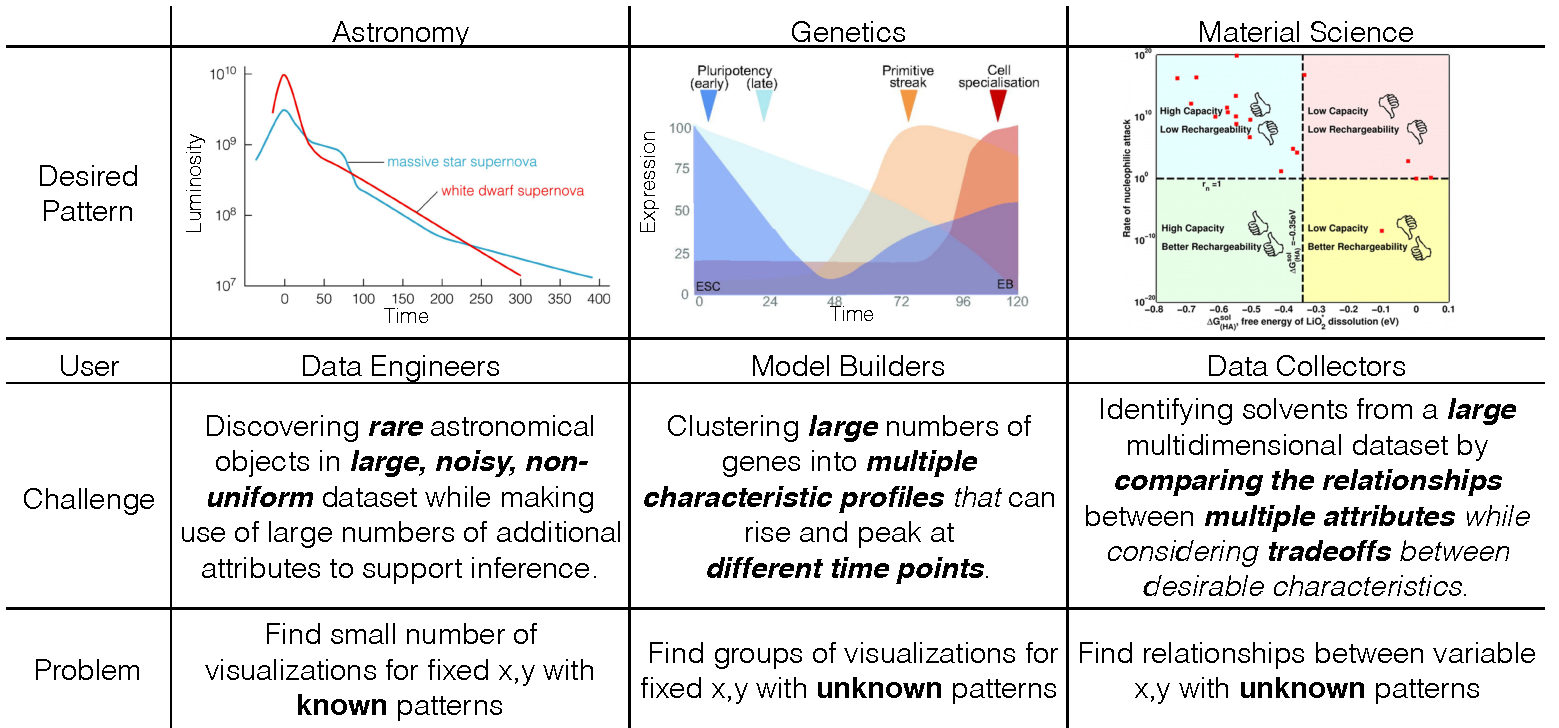
\includegraphics[width=0.8\linewidth]{figures/sci_challenge_tbl.pdf}
% \vspace{-6pt}\caption{Descriptions of the three scientific use cases discussed in this paper.}
% \label{example}
% \vspace{-10pt}
% \end{figure*}

% \noindent \emph{RQ2: What types of interface capabilities are necessary to develop VQSs into a useful component of data analysis?}
% \par Via participatory design, we distilled 
% \tvcg{Based on our early interactions with scientists,
% we started to build a VQS~\cite{Siddiqui2017VLDB,Siddiqui2017} that, similar to existing VQSs~\cite{wattenberg2001sketching}, allowed them to search for desired trends via drawing on a canvas. This early system served as a functional prototype for us to engage with scientists further in the participatory design process, understand how they envision themselves using a VQS, and gather feedback on feature designs that could make the VQS more useful. The features we developed address challenges shared across the three scientific domains, ranging from additional querying modalities, to features that support a more integrated workflow, to improving the interpretability of the system output, \tvcg{most of them missing in} prior VQSs in the literature. Our collaborative design experience culminated in a full-fledged VQS, \zv, capable of facilitating rapid hypothesis generation and insight discovery.}

% \noindent \emph{RQ3: How do VQSs accelerate scientific insights?} and \emph{RQ4: How can VQSs fit within the context of existing data analysis workflows?}
% \\ To evaluate our final system \zv, we conducted a user study with nine scientists (including those who had participated in the design process), all of whom had a vested interest in using a VQS to address their research questions on their datasets. In a 1.5-hour user study, our scientist participants were able to gain novel scientific insights, such as \emph{\tvcg{identifying a star with a transient pattern that was known to harbor a Jupiter-sized planet,} finding characteristic gene expression profiles that confirmed the results of a related publication, and learning that the dip in an astronomical light curve is caused by saturated imaging equipment overlooked by the existing error-detection pipeline}.  Participants also gained additional insights about their datasets, including debugging \tvcg{mislabelled features and uncovering the erroneous data preprocessing procedure applied to a collaborator's dataset.}
% that the way data is aggregated across multiple experiments is erroneous on a collaborator's dataset.
% We learned how VQSs could be contextualized within scientific data analysis workflows and discovered that VQSs can be used beyond the exploratory phase of analysis, for data verification, debugging preliminary datasets, and performing sanity-checks on downstream models.

% \begin{figure}[h!]
%     \centering
%     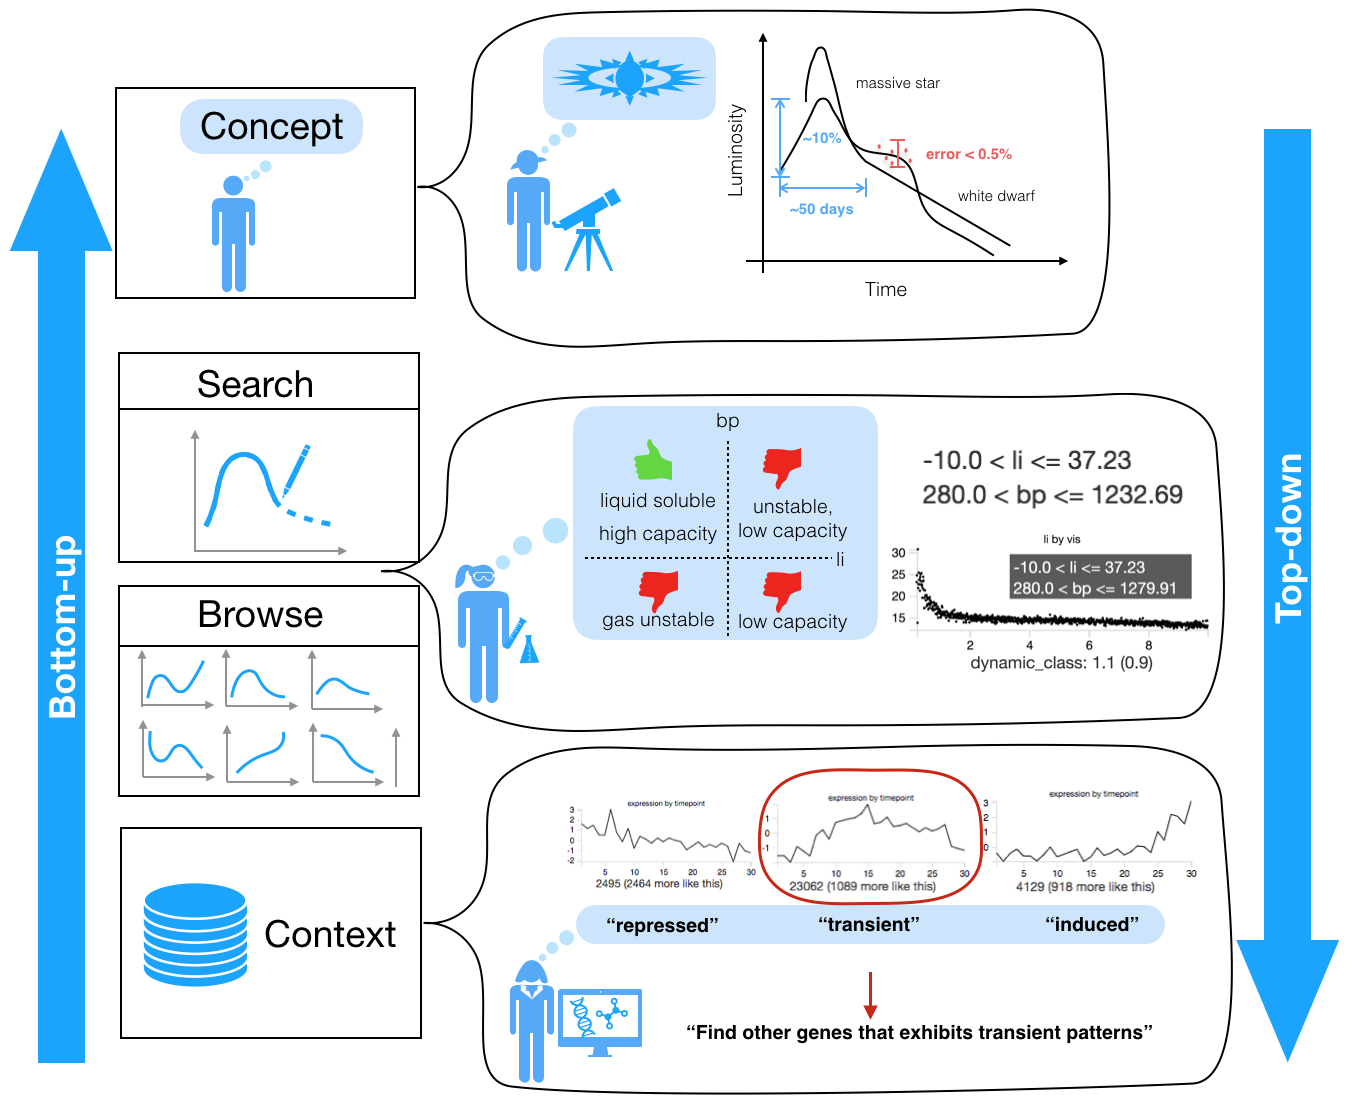
\includegraphics[width=\linewidth]{figures/search-browse-model.png}
%     \vspace{-6pt}\caption{Search Browse Model}
%     \label{fig:sbmodel}
%     \vspace{-5pt}
% \end{figure}
